\documentclass[10pt,a4paper]{article}
\usepackage[a4paper]{geometry}

\usepackage{polski}
\usepackage{xltxtra}
\usepackage{indentfirst}
\usepackage{relsize}
\usepackage{fancyvrb}
\usepackage[pdfborder={0 0 0}]{hyperref}
\usepackage{graphicx}
\usepackage{changepage}

%% tweak fonts
\defaultfontfeatures{Mapping=tex-text}
\setromanfont{Charis SIL}
\setsansfont[Scale=MatchLowercase]{Helvetica Neue}
\setmonofont[Scale=MatchLowercase]{Menlo}
\linespread{1.25}

%% define custom commands and environments
\DefineVerbatimEnvironment%
  {SmallVerbatim}%
  {Verbatim}{fontsize=\relsize{-0.5},numbers=left,numbersep=-10pt,frame=lines,tabsize=4}

\newcommand{\f}[1]{\texttt{#1}}
\newcommand{\s}[1]{\textsf{#1}}

\begin{document}

%%fakesection{Tytuł}
\title{
  Sprawozdanie nr~3 z~laboratorium\\Podstaw Inżynierii Oprogramowania
}
\author{
  Grzegorz Bartkowiak\\
  Tomasz Cudziło\\
  Mateusz Ochtera\\
  Gustaw Wypych\\
  \\
  \textsc{PW EE Informatyka}\\[10pt]
}
% \date{\today}
\date{9 maja 2011}
\maketitle

\section{Diagram klas}

Diagram klas znajduje się na stronie \pageref{fig:diagram_klas}. Zależności
między klasami są stosunkowo nieskomplikowane i~pozwalają na łatwą rozbudowę
systemu.

\subsection{Użytkownicy}

Główne klasy reprezentujące użytkowników systemu to \s{Client} i~\s{Employee}.

\subsubsection{Autentykacja}

Klasy te dziedziczą po \s{User}, która jest abstrakcyjna i~zawiera logikę
odpowiedzialną na autentykację użytkowników lub pracowników. 

\subsubsection{Autoryzacja}

Dodatkowo, posiada one referencję do obiektu klasy \s{Authorization}
określające uprawnienia użytkownika. Logika autoryzacji jest dosyć prymitywna.
Składa się na nią typ wyliczeniowy z~akcjami możliwymi do wykonania w~systemie.
Metodą \f{can()} zwraca wartość \f{true} gdy dana instancja \s{User} ma prawo
wykonać podaną jej akcję.

Minusem takiego rozwiązania jest konieczność pamiętania przez programistę do
wywoływania tej metody kiedy zachodzi taka potrzeba. Rozwiązaniem byłoby
wykorzystanie wzorca \s{Proxy}. \s{User} odwołując się do \s{Auction} albo
\s{Item} przechodziłby przez pośrednika, który w~zależności od wartości
zwróconej przez metodę \f{can()} odrzucałby prośbę, albo przekazywał ją dalej.

\subsubsection{Administrator}

Klasa \s{Administrator} jest wyspecjalizowanym pracownikiem, który pomija
proces autoryzacji tzn. może dokonać wszelkich zmian. Odpowiednik \f{root}.
Posiada również metody zarządzające całym systemem, np. włączenie trybu
konserwacji.

\subsection{Przedmioty}

Reprezentacją przedmiotów jest klasa \s{Item}. Posiada jednego właściciela i~co
najmniej jednego nadzorcę. Przedmiot obsługiwany jest różnie w~zależności czy
został właśnie dostarczony do domu aukcyjnego, czy jest wystawiony na aukcji
czy może został już sprzedany. Dlatego klasa \s{Item} jest zaimplementowana
według wzorca \s{State}. Pozwala to na dynamiczną zmianę zachowania przedmiotu
w~zależności od akcji podjętych przez użytkowników.

\subsection{Aukcje}

Klasa \s{Auction} jest centralnym punktem systemu. Poza standardowymi
odniesieniami do klientów związanych z~nią w~różnych rolach, zawiera również
informacje o~płatnościach i~wysyłce przedmiotu.

Klasy odpowiadające za obsługę płatności i~wysyłki są zaimplementowane według
wzorca \s{Strategy}. Wygodny sposób na obsługę wielu różnych algorytmów. Każdy
rodzaj płatności lub wysyłki ma identyczny interfejs, jednak ich implementacje
są różne. Ułatwia to również dodawanie nowych sposobów płatności~--- wystarczy
stworzyć tylko nową klasę z~interfejsem \textit{\s{PaymentMethod}}.

\begin{figure}[p]
  \begin{adjustwidth}{-3cm}{-3cm}
    \centering
    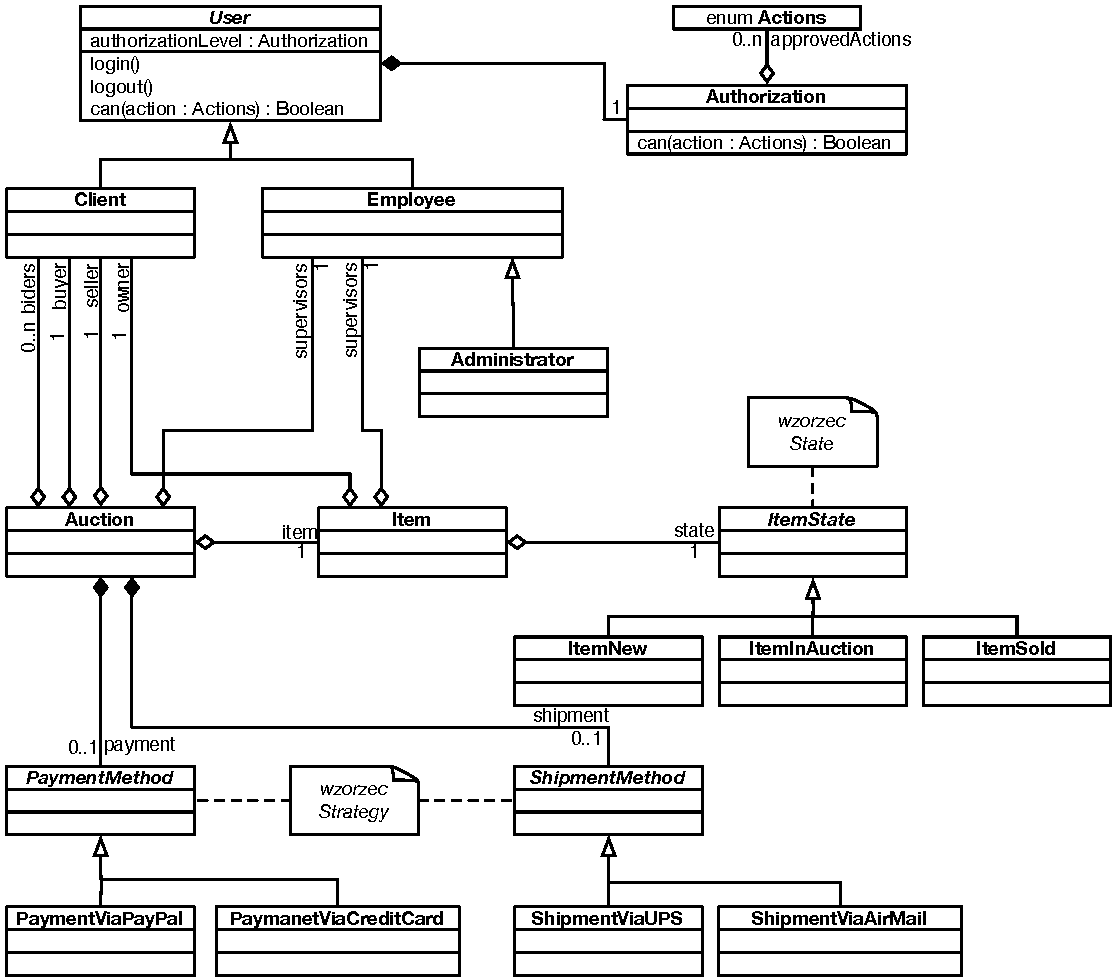
\includegraphics{figury/diagram-klas}
    \caption{Schemat klas.}
    \label{fig:diagram_klas}
  \end{adjustwidth}
\end{figure}

\newpage
\section{Logiczny model danych}

Schemat danych znajduje się na rys.~\ref{fig:model_danych} na
str.~\pageref{fig:model_danych}. Modele zawierają tylko najistotniejsze
elementy z~punktu funkcjonowania systemu.

\subsection{Użytkownicy}

\noindent Najważniejszymi tabelami są \s{Clients} i~\s{Employees}. Każda z~nich
zawiera informacje:

\begin{itemize}
  \item osobiste~--- tabela \s{PersonalData},
  \item potrzebne do zalogowania się do systemu~--- tabela
    \s{AuthenticationData},
  \item pracownicy dodatkowo informację o~poziomie uprawnień~--- tabela
    \s{AuthorizationData}.
\end{itemize}

Informacje te zostały wydzielone by uniknąć powtarzających się kolumn
w~tabelach użytkowników i~pracowników. Dodatkowo ułatwia to rozwijanie systemu
w~przyszłości, np. przystosowanie systemu do korzystania z protokołu OAuth.

Tabela \s{AuthorizationLevels} jest tabelą stałą, zapełnioną możliwymi
poziomami uprawnień przewidzianymi przez system.

\subsection{Aukcje}

Model aukcji jest bardziej skomplikowany, posiada zależności do wielu elementów
systemu. Tabela \s{Auctions} posiada odniesienia do klienta, który wystawił
przedmiot, oraz który ewentualnie kupił przedmiot. Pamięta historię licytowania
pośrednio przez tabelę \s{Bids}. Posiada też informację o~pracownikach je
nadzorujących oraz o~wystawionym przedmiocie.

Tabela aukcji powinna zawierać kolumnę z~wartością ostatniej oferty. Jest to
powtarzanie wartości z~tabeli \s{Bids}, jednak znacznie odciąży bazę danych.
Tabela \s{Bids} zapełnia się bardzo szybko i~posiada znacznie więcej wierszy
niż tabela \s{Auctions}, nawet przy dobrze dobranych indeksach na tabeli zysk
czasowy powinien być znaczący.

Przedmiot (tabela \s{Items}) pamięta, w~których aukcjach przedmiot brał udział
jeśli nie został sprzedany wcześniej. Koniecznie posiada referencję do
właściciela i~co najmniej jednego opiekuna.

Kolumny tabeli z~informacjami o~płatnościach i~wysyłce są uzależnione od
zewnętrznych systemów fiskalnych i~spedycyjnych wykorzystywanych przez dom
aukcyjny. Muszą na pewno zawierać odniesienie do aukcji, której dotyczą,
a~pośrednio przez nią informacje o~klientach i~przedmiocie aukcji.

\begin{figure}[p]
  \begin{adjustwidth}{-2cm}{-2cm}
    \centering
    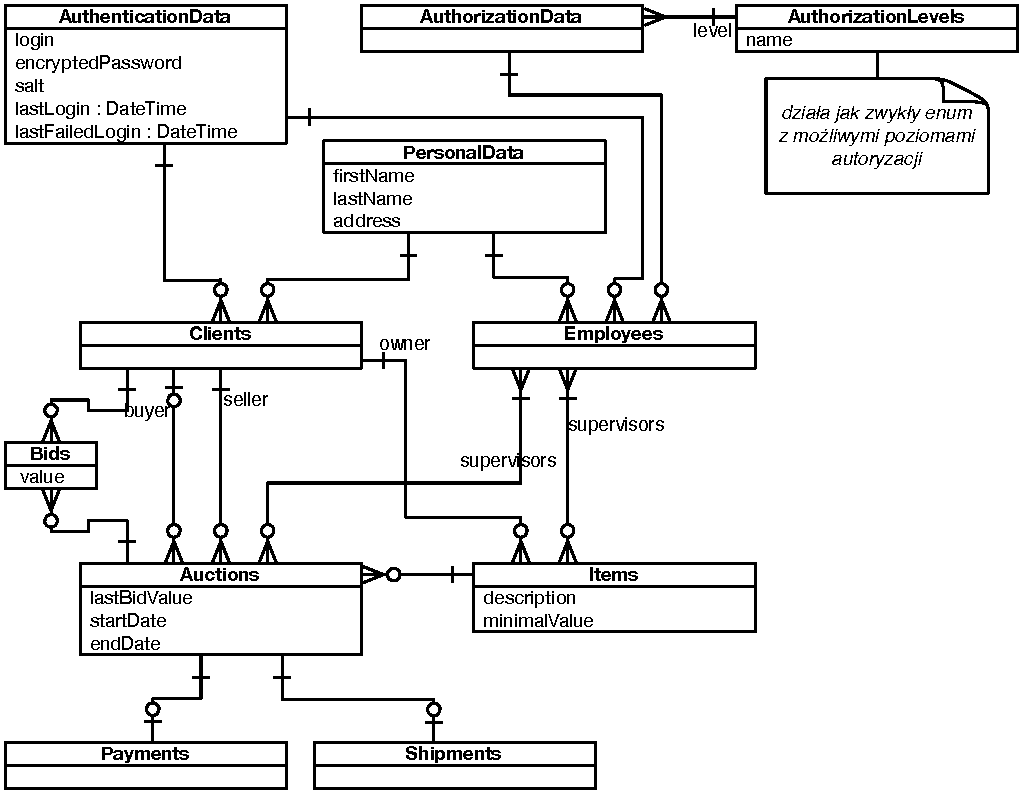
\includegraphics{figury/model-danych}
    \caption{Schemat modelu danych.}
    \label{fig:model_danych}
  \end{adjustwidth}
\end{figure}

\newpage
\section{Diagramy aktywności}

\end{document}

